\definecolor{gray}{gray}{0.6}
\section{Sprint 2}

\subsection{Sprint Planning}
	In this sprint the group is planning on a big delivery. In the last sprint the group
	implemented the fundamental structure in the game, such as models, presenters and views. 
	The implementations in the last sprint was crucial for this sprint in order to 
	be able to implement a lot of game logic to make the game more "playable".

	The group will focus on the requirements with critical and high priority in order
	to deliver as promised. There should be no critical requirements left at the end of 
	the sprint, and only a few requirements with a high priority. There will also be more 
	focus on the implementation, rather than writing more content to the report.

	At the end of the sprint, we will also use time testing what has been implemented.
	The tests will ensure that the functions that have been implemented works as planned 
	and that the product is ready for the sprint delivery with the customer. The testing is 
	done manually because there will not be time to implement unit tests in this sprint.

	During the sprint, the group members need to focus more on the workload because we did
	not manage to reach the workload expected from the course staff. This is crucial
	for the group in order to be able to deliver the product and meet the deadlines.

\subsection{Duration and Workload}
	In the last sprint, we did not reach the workload expected by the course staff.
	In the start of the sprint, the scrum master made timetable together with the
	scrum team in order to ensure more workload. The goal was to at least have an
	average workload pr/person to be 25 hours pr/week. 

	{\bf Duration:} 30.09 - 13.10 (2 weeks)\\
	{\bf Workload:} This is the list with hours spent (the whole group) on the project in this sprint.
	\begin{itemize}
		\item {\bf Planning:} 11 hours
		\item {\bf Development:} 85 hours
		\item {\bf Design:} 0 hours
		\item {\bf Documentation (report):} 65 hours
		\item {\bf Testing:} 3.5 hours
	\end{itemize}
	{\bf Total workload: } 165 hours \\

	The group's goal was to work at least 20-25 hours pr/person every week in this sprint. 
	We did manage the workload, and we had a avrage of 20.6 hours/week (165 hours/4 persons/2 weeks = 20.6 hours). 
	The scrum master have the responsibility to ensure that the workload is met with the
	expectations from the course staff, and we managed it in this sprint.
	The changes from the last sprint is that we worked late hours and used the weekend effective
	since the entire group is occupied with UKA, voluntary work and homework.

\subsection{Sprint Backlog}

	In this sprint we planned to implement the most of the requirements with critical and high
	priority. In the start of the sprint we only planned to implement 8 requirement, but
	during the sprint we manage to implement them and added more requirements to the sprint backlog.
	In the end of the sprint the backlog consisted of a total of 15 requirements. Here are the
	sprint backlog from this sprint:

	\begin{table}[H]
	\begin{tabular}{| p{1cm} | p{7cm} | p{2cm} | p{2cm} |}
		\hline
		\rowcolor{gray}
		ID & Description & Estimate & Actual effort \\ \hline
		FR1.1 & The user should be able to read game instructions from the main menu
		& 2 hours & 2 hours \\ \hline

		FR1.12 & The user should not get the opportunity to tilt the screen by tilting the phone. 
		& 3 hours & 4 hours \\ \hline
		
		FR2.2 & The user should be able to buy and place several power stations on the game map.
		& 4 hours & 5 hours \\ \hline

		FR2.3 & The user should be able to buy and place power cables on the map. 
		& 10 hours & 11 hours \\ \hline

		FR2.4 & The user should be able to upgrade the power plant. 
		& 2 hours & 3 hours \\ \hline

		FR2.8 & The user should be able to see information about a buildings when tapping on them.
		& 3 hours & 2 hours \\ \hline

		FR3.6 & When an existing building is not supplied with power within a certain amount of time, 
		the house should disappear and the player's health score should decrease. 
		& 8 hours & 6 hours \\ \hline

		FR4.2 & The user should be able to continue a level while the health score is greater than zero. 
		When the health score reaches zero, the game is over. 
		& 2 hours & 1 hour \\ \hline

		FR5.1 & The user should be able to collect money from the buildings connected to the power plant
		& 5 hours & 4 hours \\ \hline

		FR5.2 & When connecting buildings through power cables, there should be a cost which is 
		proportional to the length of the cable. 
		& 5 hours & 6 hours \\ \hline

		FR5.3 & It should cost money to upgrade the power plant. 
		& 2 hours & 2 hours \\ \hline

		FR6.3 & The user should be able to click on a power plant to receive information about 
		the cost of upgrading it and what the upgrade does. 
		& 3 hours & 4 hours \\ \hline

		FR6.7 & The user should be able to see the main menu when he or she starts the game. 
		& 4 hours & 8 hours \\ \hline

		FR6.8 & When the player wants to place a power plant or a power cable in building mode, 
		the player should be prompted if they want to go through with it, or cancel. 
		& 4 hours & 3 hours \\ \hline

		FR6.9 & The user should be able to see that he or she is in building mode when selecting 
		a building to build in the hub menu. 
		& 9.5 hours & 14 hours \\ \hline

		FR6.10 & The user should be able to see that a building has gone without power for 
		some time, and is affecting the player's health score if the building is not connected 
		to a power plant before it disappears. 
		& 8 hours & 10 hours \\ \hline
	\end{tabular}
	\caption{Sprint backlog sprint 2}
	\end{table}

\subsection{Implementation}
	
	This is the actual implementation of requirements that we managed to implement
	from the sprint backlog.
	
	\begin{itemize}
		\item {\bf Building mode:} When the player open the hud (menu in the bottom of the screen) and presses
		on the build powerplant/powercable image, the player enters the building state 
		"build powerplant/build powerlines". The game state is set back to normal after the player 
		is finished with the building. The game has a state variable that contains which mode the 
		game is in (Normal, build power plant or build power lines). When the player is in the building
		state, two lines will appear (on top and bottom) on the screen that looks like constructions mode
		(yellow and black stripes). The look and feel is important for the user to understand that
		the game-state is changes to building mode. 

		\item {\bf Upgrade power plants:} When the player taps on the power plant, a pop-up will appear.
		In the pop-up it will show the level the power plant is in and how much it will cost the 
		player to upgrade the power plant. If the player choose to upgrade the power plant the level will
		increase by 1. If the player do not want to upgrade, he or she press "cancel" and the player will be sent
		back to the game. The part that is not implemented here is that when a power plant is upgraded, 
		it will be able to serve more buildings with power and this should also be added to the building 
		information in the pop-up. If the player does not have enough money, the player gets a message 
		that he or she cannot upgrade.

		\item {\bf Building and buy power plants:} When the player open the menu in the bottom and 
		choose the "build powerplant" icon, the player enters the building mode and is able to 
		tap on the screen where he or she wants to place the power plant. When the player taps on the
		location to place the building, it will a appear a pop-up with the question if the player 
		want to buy and build the power plant. If the player want to build the power plant, a certain
		amount of money will be payed from the players money or if the player press "cancel", the 
		game goes out of the building state and back to normal. If the player choose to buy the 
		power plant, but do not have enough money, the player get a message that he or she do not have
		enough money and the game state will be set back to normal. 

		\item {\bf Connect buildings to power plants:} When the player open the menu in the bottom and 
		choose the "build powerline" icon, the player enters the building mode and the player is able
		to build power lines. The power lines is build by tapping on the desired en-points (house-house 
		or house-power plant).

		The part that is not implemented is the logic for handling the "connection state" of a building, 
		as well as the amount of power a power plant can serve. It is not implemented that if the building
		is connected, the countdown will stop and make money that the player can collect. The money should
		only be "produced" if the building is connected to a power plant. The amount of money that is 
		produced should be building specific because different buildings use different amount of power, and
		therefore need to pay a different amount of money. 

		\item {\bf Collect money:} When a building is connected to another building, it starts 
		"producing" money. The building will show a icon of a coin when the player is able to 
		collect the money. The money is collected when the user taps on the building with a coin. 

		The parts that is missing is that it needs to check whether the connected building is a power plant 
		or just another building. It should only produce money if it is connected to a power plant. 
		If the building have produced money, a coin will appear on the building. When the player tap
		on a building with a coin icon, it will collect the money and the players amount of money 
		will increase. 

		\item {\bf Game over:} When the health bar is zero, the game is over and the game over screen 
		is showing. When the player press "ok", the player is sent to the main menu and is able to 
		start a new game. This part may need some changes to the look and feel, but it is working.

		\item {\bf Main menu:} When the game is starting, the app is showing the main menu. 
		From this menu, the player is able to choose between "Start game", "Instructions" and high score.

		\item {\bf Money and goal:} When the player has started the game, the score and goal for
		the level is showing in the hud. To get to the next level, the player need to get the same
		amount of money as the goal in order to go to the next level. The logic for the level
		is not finished yet.

		\item {\bf Information about power plant:} If the user taps on a power plant it will pop up
		information about the power plant like level and upgrade information. It is not implemented yet,
		but it will be implemented more information like how much power it can serve and how mange
		buildings that are connected. 

		\item {\bf Health bar:} In the bottom of the game it is showing a health bar. If the 
		health bar is below zero, it is game over, so the player need to keep track of the health.
		A user loses health if a new buildings countdown is over and the building disappears.
		The health bar will send a signal with a color. If the player has full health bar the bar is
		green, then it gets orange and in the end it is red. 

		\item {\bf Countdown on building:} when a building appear, a countdown starts. If the player
		do not connect the building to a power plant, the countdown wont stop. If the countdown is
		finished, the house will disappear and the health bar will decrease. This is a signal to
		the player so he or she is able to connect the building to a power plant in order to not loose
		health. 

	\end{itemize}

	This is the requirements that was in the sprint backlog that we did not
	manage to finish and have removed to sprint 3:

	\begin{itemize}
		\item {\bf Information about building:}

		\item {\bf The cost of the power lines:}

	\end{itemize}

	\begin{figure}[H]
	\centering
	\subfigure{
		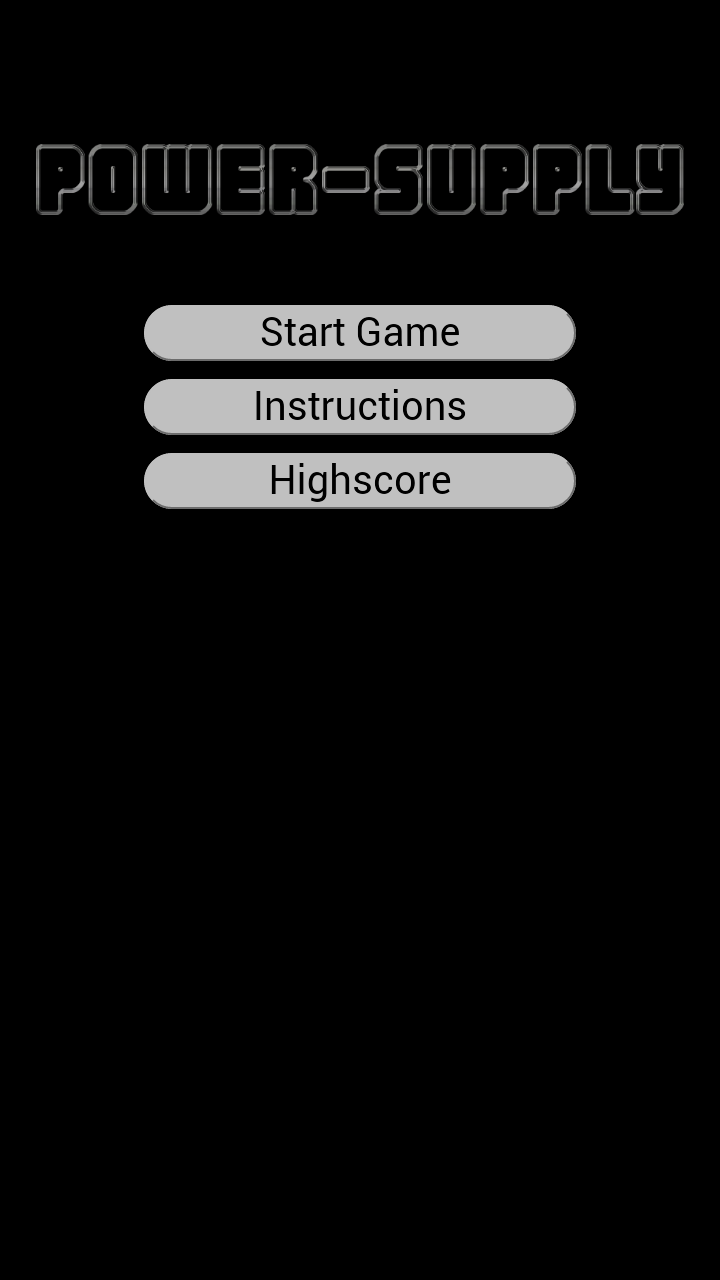
\includegraphics[scale=0.17]{pictures/sprint2-screen/sprint2-2}
	}
	\subfigure{
		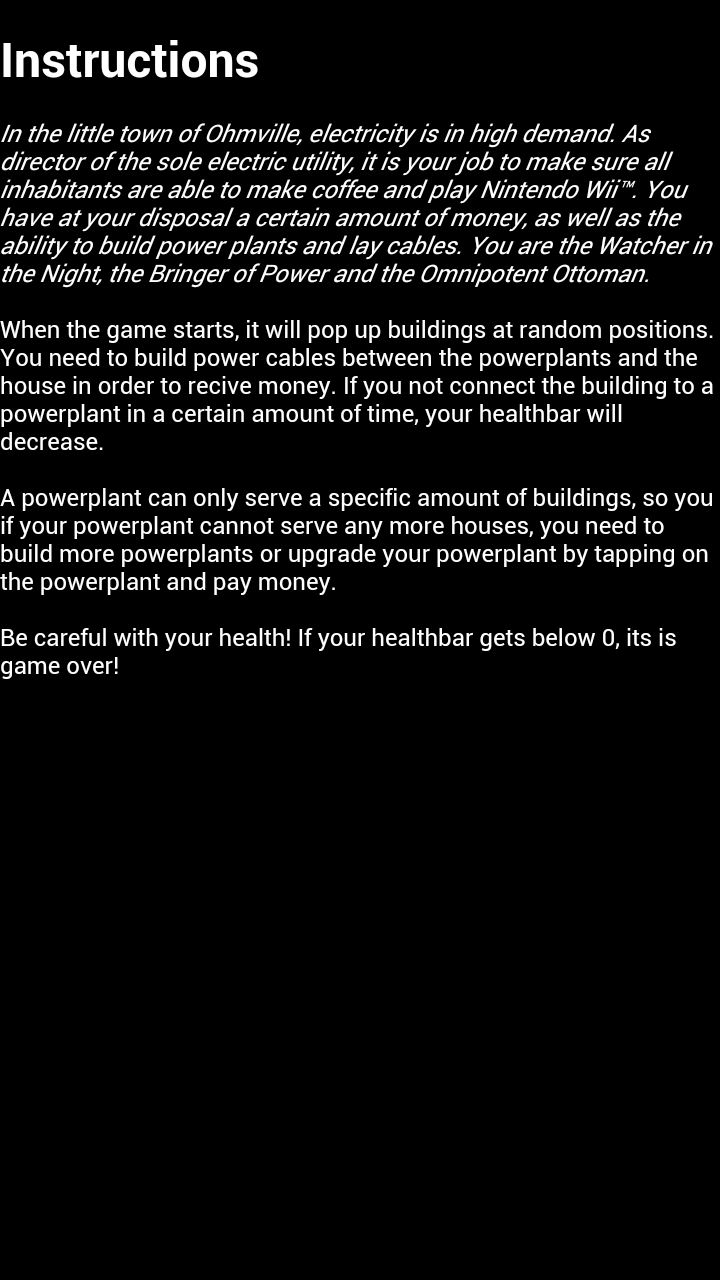
\includegraphics[scale=0.17]{pictures/sprint2-screen/sprint2-3}
	}
	\caption{Main menu and instruction screen}
	\end{figure}

	\begin{figure}[H]
	\centering
	\subfigure{
		
\includegraphics[scale=0.17]{pictures/sprint2-screen/sprint2-4}
	}
	\subfigure{
		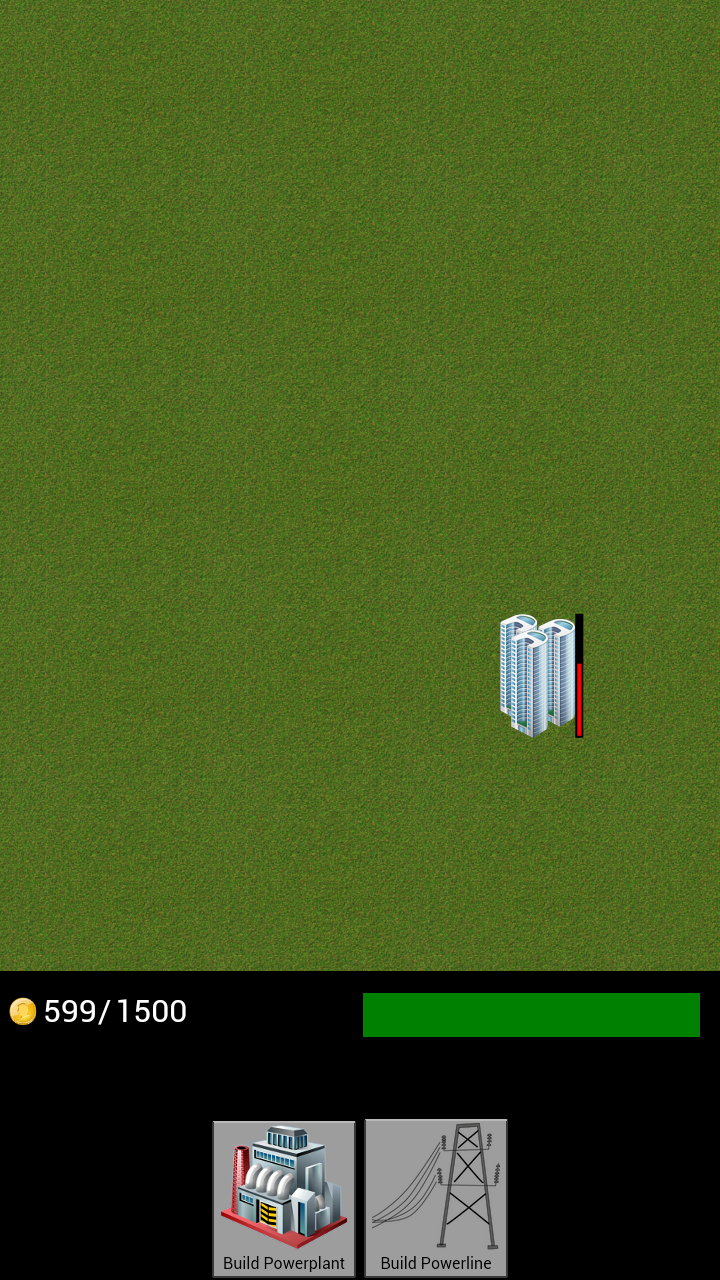
\includegraphics[scale=0.17]{pictures/sprint2-screen/sprint2-5}
	}
	\caption{Ingame headsup display (hud)}
	\end{figure}

		\begin{figure}[H]
	\centering
	\subfigure{
		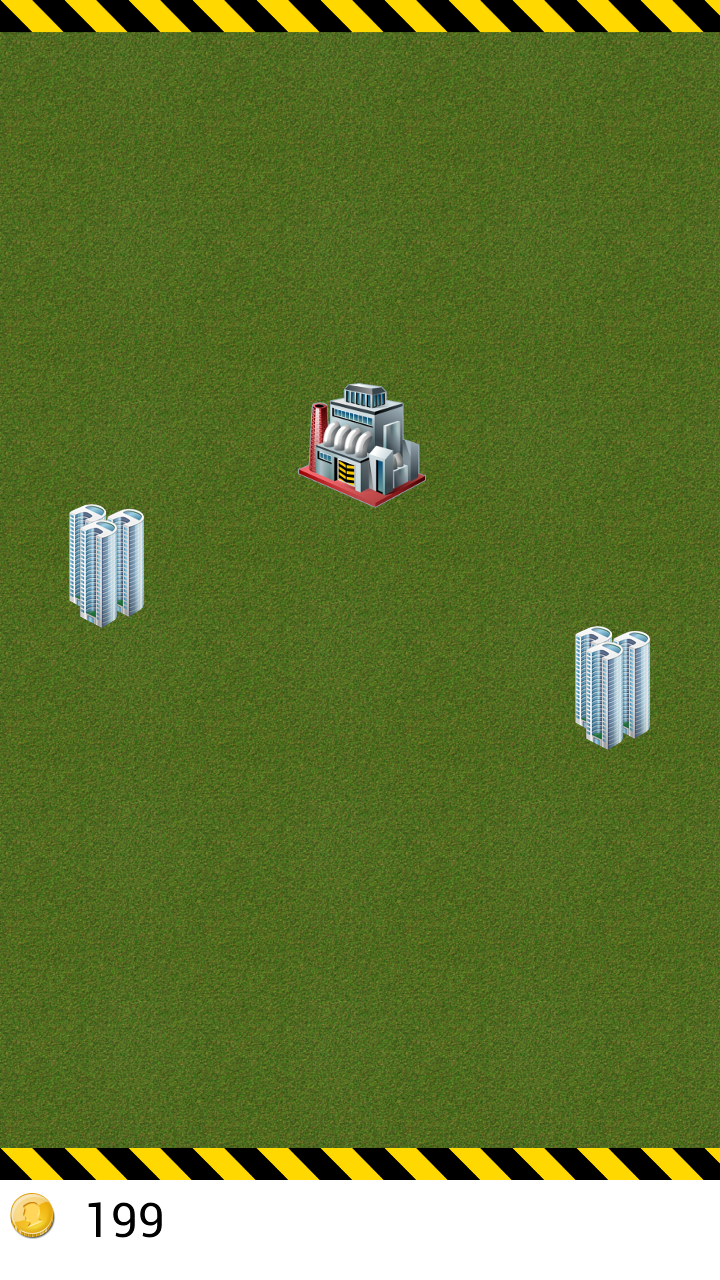
\includegraphics[scale=0.17]{pictures/sprint2-screen/sprint2-1}
	}
	\subfigure{
		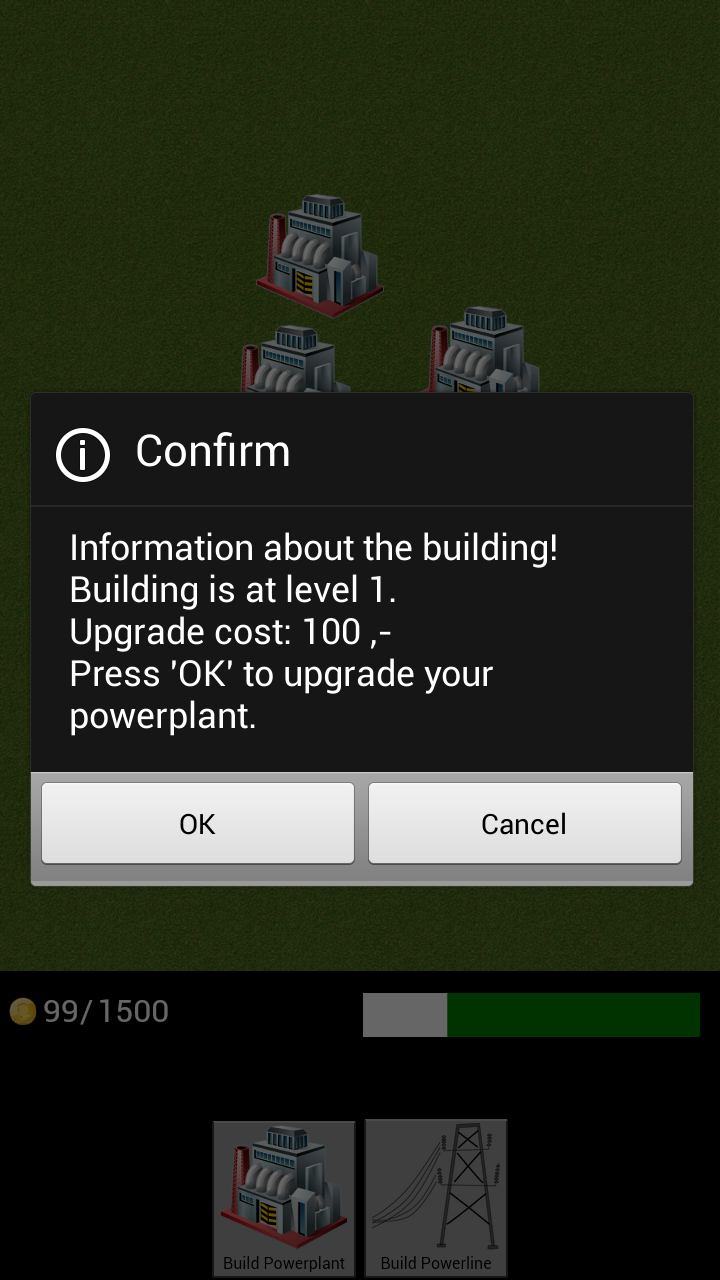
\includegraphics[scale=0.17]{pictures/sprint2-screen/sprint2-12}
	}
	\caption{Building Powerplants}
	\end{figure}

	\begin{figure}[H]
	\centering
	\subfigure{
		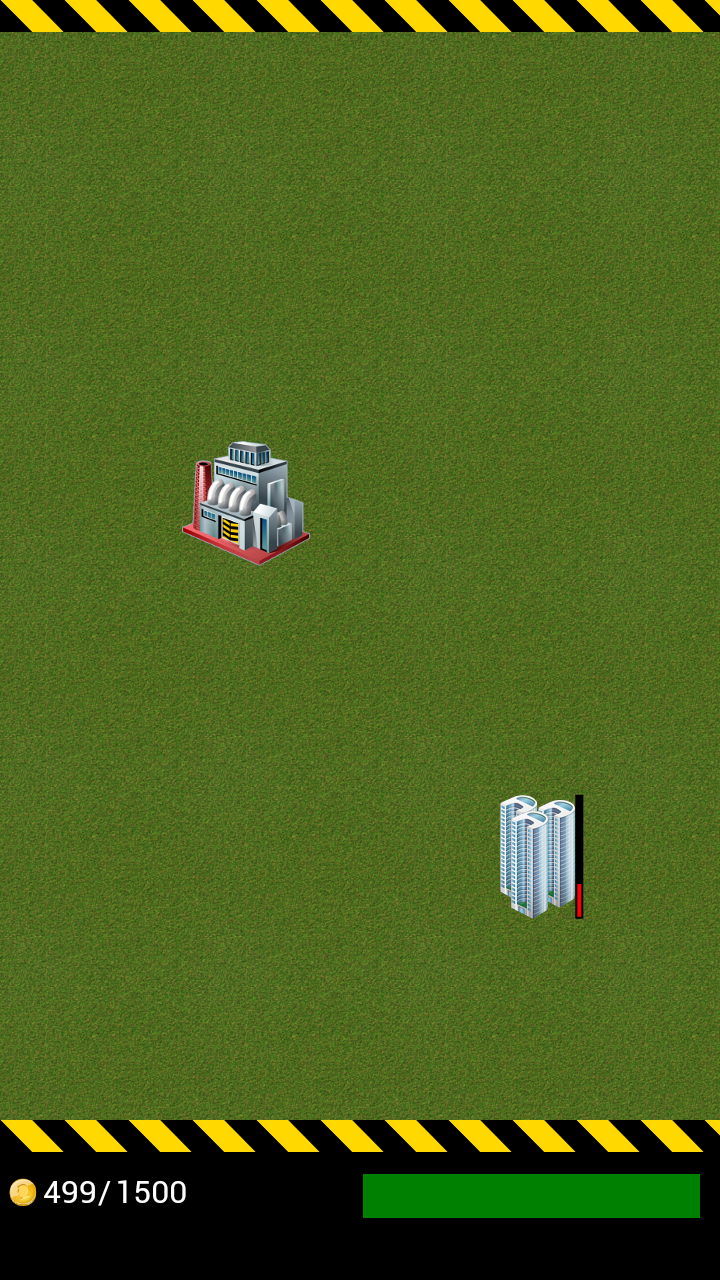
\includegraphics[scale=0.17]{pictures/sprint2-screen/sprint2-6}
	}
	\subfigure{
		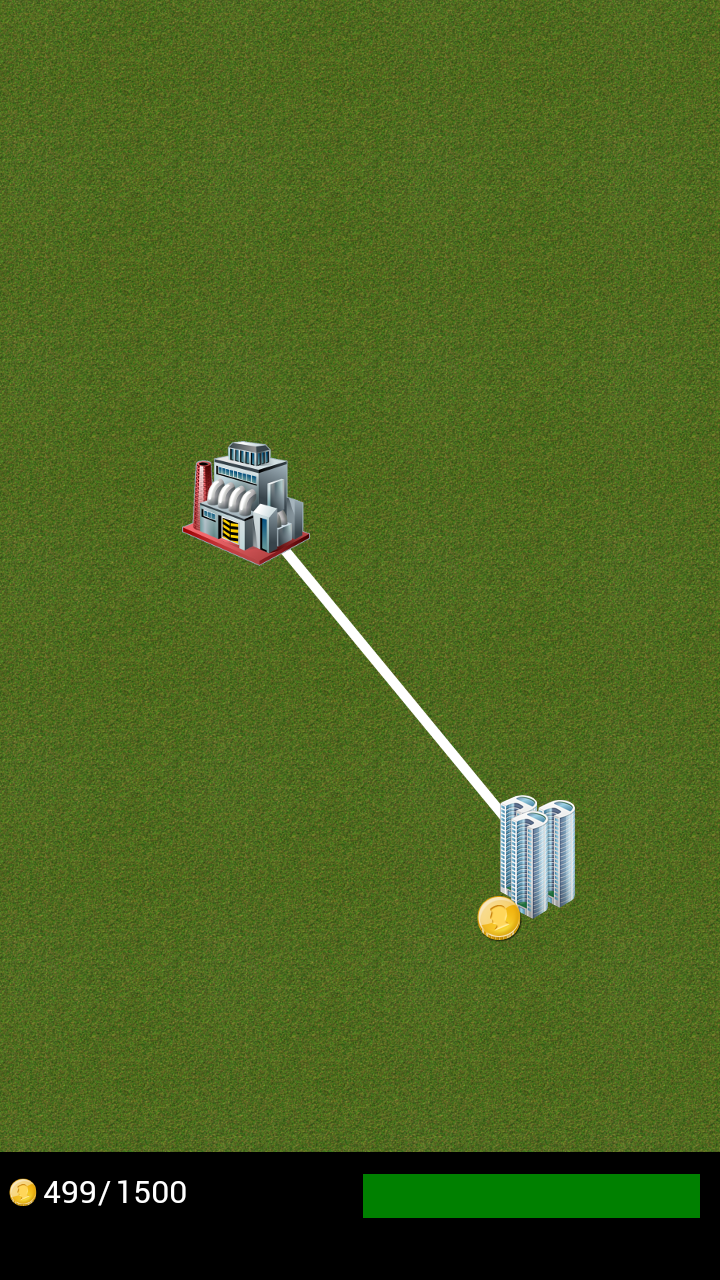
\includegraphics[scale=0.17]{pictures/sprint2-screen/sprint2-7}
	}
	\caption{Building Powerlines}
	\end{figure}

		\begin{figure}[H]
	\centering
	\subfigure{
		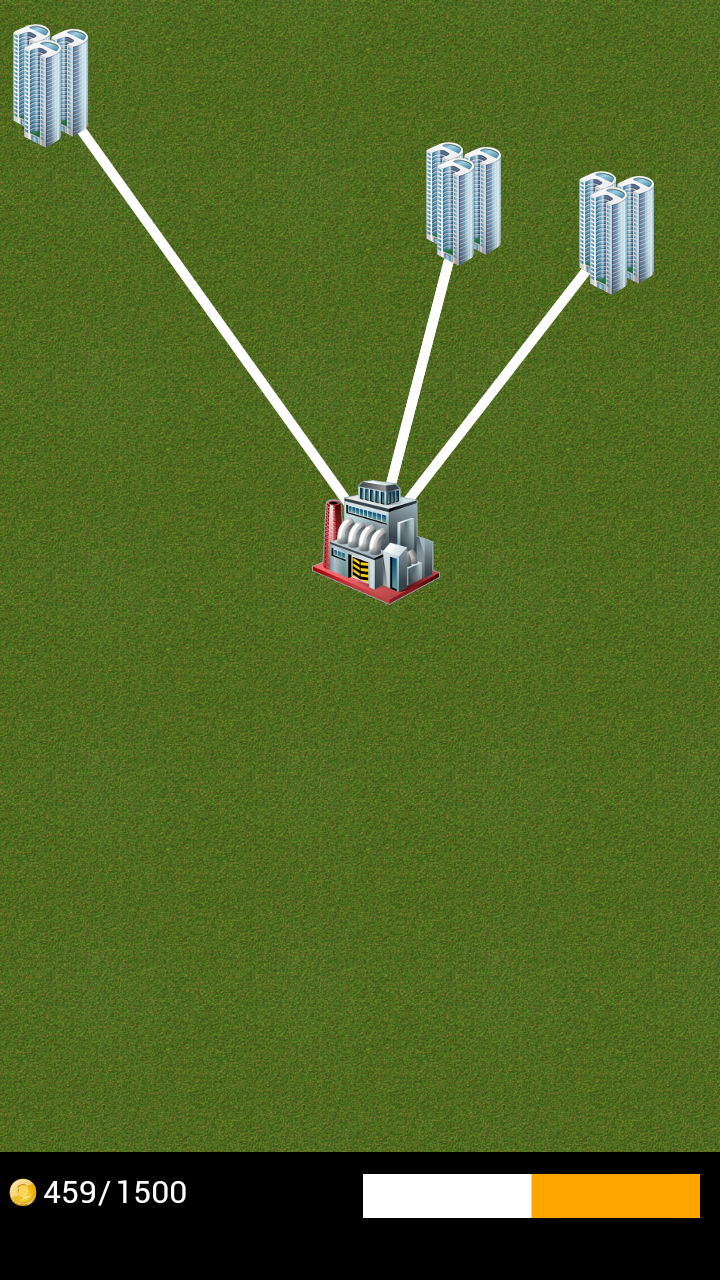
\includegraphics[scale=0.17]{pictures/sprint2-screen/sprint2-8}
	}
	\subfigure{
		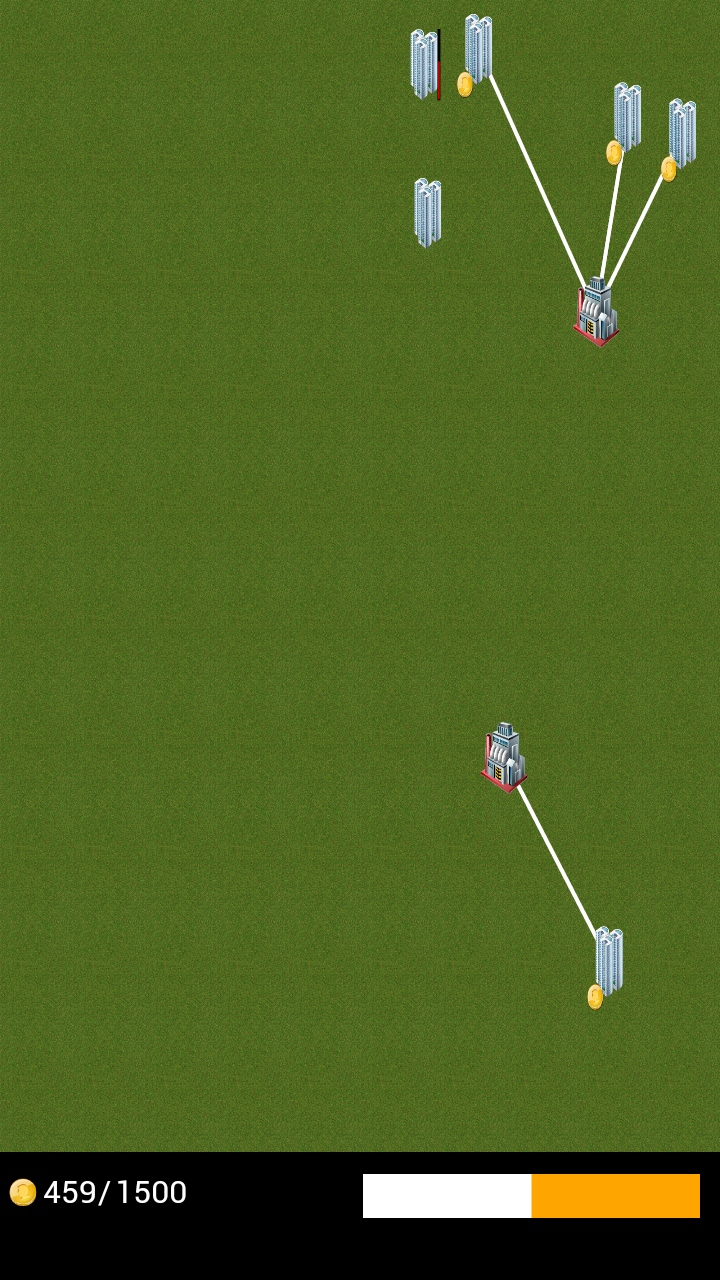
\includegraphics[scale=0.17]{pictures/sprint2-screen/sprint2-9}
	}
	\caption{Connecting multiple buildings}
	\end{figure}

	\begin{figure}[H]
	\centering
	\subfigure{
		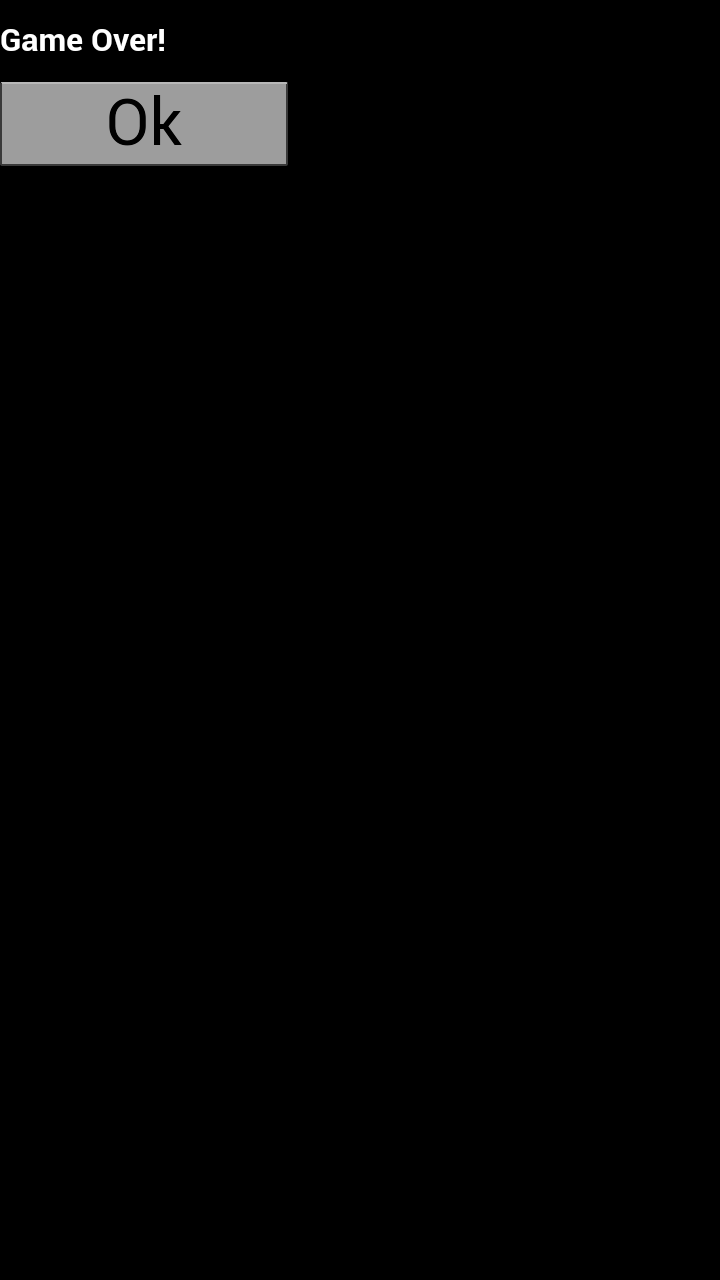
\includegraphics[scale=0.17]{pictures/sprint2-screen/sprint2-10}
	}
	\subfigure{
		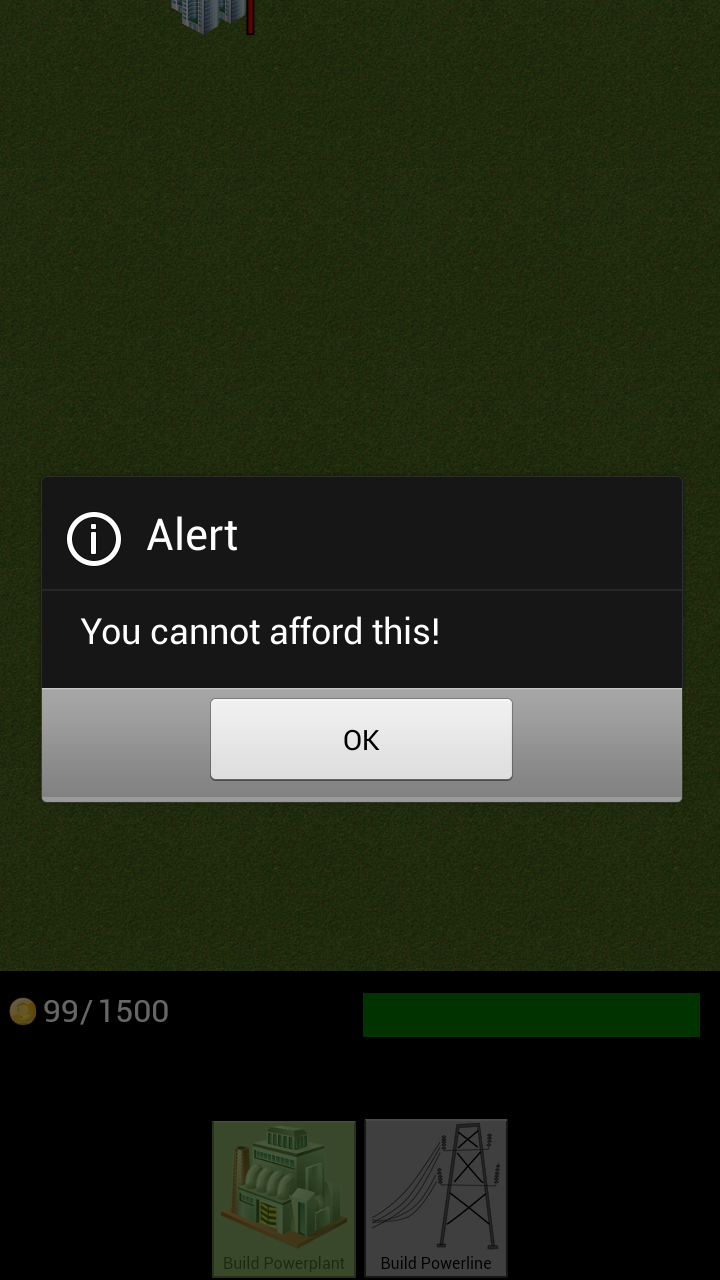
\includegraphics[scale=0.17]{pictures/sprint2-screen/sprint2-11}
	}
	\caption{Game over screen and ingame alerts}
	\end{figure}

\clearpage
\subsection{Testing}

	\subsubsection{Tests Introduced in this Sprint}

	The functional tests executed in this sprint are listed here. The test cases can be found in chapter 7.4.

	\definecolor{lightgray}{gray}{0.9}

	\begin{table}
	\begin{tabular}{| p{3cm} | p{6.5cm} | p{2.5cm} |}
		\hline
		\rowcolor{lightgray}
		{\bf Test Case} & {\bf Result} & {\bf Pass/Retest} \\ \hline
	  	
	  	FT-04 Main Menu & Works as expected. & Pass. \\ \hline

		FT-05 Build Power Plants & It is still possible to build on top of other buildings, otherwise it works as expected. Needs minor adjustment. &  Retest. \\ \hline

		FT-06 Build Power Lines & Building power lines is currently free, it is possible to connect a building to several power plants, and power lines may cross each other. Otherwise it works as expected. Needs adjustments.  & Retest. \\ \hline

		FT-07 Upgrade Power Plant & Upgrading a power plant does not yet affect the amount the power plant can supply. This will be implemented at a later stage. & Retest. \\ \hline

		FT-08 Information on Power Plants & Correct information is displayed when tapping a power plant & Pass.\\ \hline

		FT-09 Building Mode & Works as expected & Pass. \\ \hline

		FT-10 Tilting & Works as expected & Pass. \\ \hline

		FT-11 Collect Money & Works as expected & Pass. \\ \hline

		FT-12 No Power and Health Bar & Works as expected & Pass. \\ \hline

		FT-13 Game Over & Works as expected. & Pass. \\ \hline

	\end{tabular}
	\caption{Functional tests from sprint 2}
	\end{table}

	\subsubsection{Redone Tests}

	The following are the tests that has been executed again this sprint, because they did not pass last sprint:

	\begin{table}
	\begin{tabular}{| p{3cm} | p{6.5cm} | p{2.5cm} |}
		\hline
		\rowcolor{lightgray}
		{\bf Test Case} & {\bf Result} & {\bf Pass/Retest} \\ \hline

		FT-02 Appearance of buildings & Buildings appear at a more controlled rate and now has the ability to disappear. But they can appear on top of each other. Needs some minor adjustments. & Retest. \\ \hline

	\end{tabular}
	\caption{Redone tests in sprint 2}
	\end{table}

\subsection{Changes to the Requirements}
	
	After the sprint 1 delivery, the group had hoped that the customer would make 
	changes to the requirement specification by either adding or removing requirements, 
	but this did not not happened. During the implementation in this sprint, the 
	team came up with several changes to the requirements. Some requirements have been moved, 
	changed, split or removed. At the end of sprint 2 we had reached version 3 of the requirement 
	specification. The changes are listed in the tabled below.

	\begin{table}
	\begin{tabular}{| p{1.5cm} | p{12cm} |}
		\hline
		\rowcolor{lightgray}
		{\bf FR} & {\bf Change} \\ \hline
		FR3.3 & {\bf \color{green} [NEW]} There should be several types of buildings on the map, 
		with different power requirements  \\ \hline
		FR3.4 & {\bf \color{green} [NEW]} Different types of building should reward different amounts of 
		money \\ \hline
		FR3.6 & {\bf \color{orange} [CHANGED]}changed priority from high to critical \\ \hline
		FR4.4 & {\bf \color{red} [REMOVED]} As the user reaches higher levels there should be an 
		increase in faulty power cables \\ \hline
		FR5.2 & {\bf \color{red} [REMOVED]} There should be buildings on the map for the user to 
		supply with power; new buildings should appear over time. \\ \hline
		FR5.4 & {\bf \color{red} [REMOVED]} The player should be able to suspend specific buildings' 
		power supply in order to server others \\ \hline
		FR5.5 & {\bf \color{orange} [MOVED TO GUI]} A power preservation tip should appear when the 
		user reaches a new level. \\ \hline
	\end{tabular}
	\caption{Changes to version 1 of the requirement specification}
	\end{table}

	\begin{table}
	\begin{tabular}{| p{1.5cm} | p{12cm} |}
		\hline
		\rowcolor{lightgray}
		{\bf FR} & {\bf Change} \\ \hline
		FR1.9 & {\bf \color{green} [NEW]} There should be played a sound effect when 
		the player collects money \\ \hline
		FR1.10 & {\bf \color{green} [NEW]} There should be played a sound effect when 
		the player upgrades the power plant \\ \hline
		FR1.11 & {\bf \color{green} [NEW]} There should be played a sound effect when 
		the player builds a power cable \\ \hline
		FR1.12 & {\bf \color{green} [NEW]} The user should not get the opportunity to 
		tilt the screen by tilting the phone. \\ \hline
		FR2.4 & {\bf \color{orange} [MOVED TO INCOMING/OUTGOING MONEY]} The user should 
		be able to connect the buildings to the power plants by building a power cable. 
		Building cables costs money. \\ \hline
		FR3.6 & {\bf \color{green} [NEW]} When an existing building is not supplied 
		with power within a certain amount of time, the house should disappear and the player's 
		health score should decrease \\ \hline
		FR3.6 & {\bf \color{orange} [MOVED TO GUI]} The user should be able to see 
		that a building has gone without power for some time, and is affecting the 
		player's health score if the building is not connected to a power plant before it 
		disappears. \\ \hline
		FR4.3 & {\bf \color{orange} [MOVED TO OBSTACLES]} When an existing building 
		is not supplied with power within a certain amount of time, the house should 
		disappear and the player's health score should decrease \\ \hline
		FR5.4 & {\bf \color{green} [NEW]} The user should be able to upgrade the power plant. 
		This cost money. \\ \hline
		FR6.7 & {\bf \color{green} [NEW]} The user should be able to see the main 
		menu when he or she starts the game. \\ \hline
		FR6.8 & {\bf \color{green} [NEW]} When the player wants to place a power plant 
		or a power cable in building mode, the player should be prompted if they want to 
		go through with it, or cancel. \\ \hline
		FR6.9 & {\bf \color{green} [NEW]} The user should be able to see that he or she 
		is in building mode when selecting a building to build in the hub menu. \\ \hline
	\end{tabular}
	\caption{Changes to version 2 of the requirement specification}
	\end{table}
	
\subsection{Group Dynamics}
	In sprint 1 the group had some problems with the group dynamics. 
	During this sprint we managed to work together as a group and the group dynamics
	is now very good. The changes that helped the group to work better as a group
	was the allocation of roles in the last sprint. 

\subsection{Customer Feedback}
	In this sprint the group got a feedback from the customer in the end of the sprint.
	The customer think that we are working structured and the flow of information is good.
	They are very pleased with the cooperation this far in the project.

	After the sprint meeting, the customer tested the game on a phone. The feedback on the game
	was that they had some problems with building the power lines as well as knowing how to play.
	The group will try to solve the problems until the next meeting.

	The customer is also very pleased with the requirement specification and the priorities
	that we have made. So far, the group has implemented the most of the critical and high
	priorities and the requirements left in the backlog is mainly medium/low. 

\subsection{Sprint Retrospective}
	\subsubsection*{Start doing: } 
		\begin{itemize}
			\item use branches for new features to be implemented and not implement new 
			features in the master branch.
		\end{itemize}
	\subsubsection*{Stop doing: }

	\subsubsection*{Continue doing: }
		\begin{itemize}
			\item Keep up the good team work
		\end{itemize}

